\documentclass[12pt]{article}

\usepackage[top=1in, bottom=1in, left=1in, right=1in]{geometry} 
\usepackage{graphicx}
\usepackage{setspace}
\usepackage{bm}
\usepackage{amsmath}
\usepackage{amssymb,amsmath}
\usepackage{listings}
\usepackage{titling}
\usepackage{color}
\usepackage{enumitem}
\usepackage{fancyvrb}
\usepackage{hyperref}
\usepackage{diagbox}
\usepackage{float}
\geometry{letterpaper}
\linespread{1.1}% \geometry{landscape} % rotated page geometry

\definecolor{codegreen}{rgb}{0,0.6,0}
\definecolor{codegray}{rgb}{0.5,0.5,0.5}
\definecolor{codepurple}{rgb}{0.58,0,0.82}
\definecolor{backcolour}{rgb}{0.95,0.95,0.92}
\definecolor{outcolor}{rgb}{0.545, 0.0, 0.0}

\lstdefinestyle{mystyle}{
	backgroundcolor=\color{backcolour},   
	commentstyle=\color{codegreen},
	keywordstyle=\color{magenta},
	numberstyle=\tiny\color{codegray},
	stringstyle=\color{codepurple},
	basicstyle=\footnotesize,
	breakatwhitespace=false,         
	breaklines=true,                 
	captionpos=b,                    
	keepspaces=true,                 
	numbers=left,                    
	numbersep=5pt,                  
	showspaces=false,                
	showstringspaces=false,
	showtabs=false,                  
	tabsize=2
}

\lstset{style=mystyle}
\setlength{\droptitle}{1cm}
\title{HW 5: Optimal PHEV Energy Management via Dynamic Programming}
\date{13 Apr. 2018} 
\author{Franklin Zhao \\ SID: 3033030808}

\begin{document}
	
	\maketitle
	\newcommand{\tabitem}{~~\llap{\textbullet}~~}
	\renewcommand\theequation{\arabic{equation}}
	\renewcommand{\figurename}{Fig.}
	\renewcommand\thesection{Problem \arabic{section}}
	\renewcommand\thesubsection{(\alph{subsection})}
	\onehalfspacing
	
\section{}
\subsection{}
\begin{equation}
\min_{P_{fuel}(K)}J=\sum_{k=0}^{N-1}\alpha\Delta tP_{fuel}(K)
\end{equation}
\subsection{}
The constrains are shown as follows:
\begin{equation}
P_{fuel}(k)=\frac{P_{dem}(k)-P_{batt}(k)}{\eta(P_{dem}(k)-P_{batt}(k))}
\end{equation}
The above equation just derived $P_{fuel}(k)$ and eliminated the variable $P_{eng}(k)$ as done in the lecture given the enginer power definition.
\begin{equation}
SOC(k+1)=SOC(k)-\frac{\Delta t}{Q_{cap}V_{oc}}P_{batt}(k)\ \ \ \ \ SOC(0)=SOC_0
\end{equation}
The above constraint describes the battery dynamics (in steps) with the initial condition.
\begin{equation}
SOC^{min}\leq SOC(k)\leq SOC^{max}
\end{equation}
The above constraint shows the boundaries of SOC in every steps.
\newpage
\begin{equation}
-P_{batt}^{max}\leq P_{batt}(t)\leq P_{batt}^{max}
\end{equation}
The above constraint shows the boundaries of power generation in every steps.
\begin{equation}
0\leq P_{dem}(k)-P_{batt}(k)\leq P_{eng}^{max}
\end{equation}
The above constraint shows the boundaries of the power that a vehicle can generate.
\subsection{}
Control variable: battery power $P_{batt}(k)$\\
State variable: state of charge $SOC(k)$
\section{}
\subsection{}
The value function is defined as the minimum of the fuel consumption in current time add the cost of all the fuel consumption in future steps.
\subsection{}
Principle of optimality equation:
\begin{equation}
V_k(SOC(k))=\min\{\alpha\Delta tP_{fuel}(k)+V_{k+1}(SOC(k+1))\},\ \ \ \ \ k=0,1,...,N-1
\end{equation}
with the boundary condition:
\begin{equation}
V_k(SOC(N))=0
\end{equation}
\section{}
\subsection{}
First limit is just Equation (5):
\begin{equation}
-P_{batt}^{max}\leq P_{batt}(t)\leq P_{batt}^{max}
\end{equation} 
For the second limit, From Equation (3), we know:
\begin{equation}
P_{batt}(k)=\frac{Q_{cap}V_{oc}}{\Delta t}(SOC(k)-SOC(K+1))
\end{equation}
Plugging this into Equation (5), we get:
\begin{equation}
\frac{Q_{cap}V_{oc}}{\Delta t}(SOC(k)-SOC^{max})\leq P_{batt}(k)\leq\frac{Q_{cap}V_{oc}}{\Delta t}(SOC(k)-SOC^{min})
\end{equation}
For the third limit, transforming Equation (6), the following will be derived
\begin{equation}
P_{dem}(k)-P_{eng}^{max}\leq P_{batt}(k)\leq P_{dem}(k)
\end{equation}
\subsection{}
Now let's collapse the contraints in (a) into one inequality:
\begin{equation}
\begin{array}{ll}
&\max\{-P_{batt}^{max},\frac{Q_{cap}V_{oc}}{\Delta t}(SOC(k)-SOC^{max}),P_{dem}(k)-P_{eng}^{max}\}\\\leq&P_{batt}(k)\\\leq& \min\{P_{batt}^{max},\frac{Q_{cap}V_{oc}}{\Delta t}(SOC(k)-SOC^{min}),P_{dem}(k)\}
\end{array}
\end{equation}
\newpage
\section{}
\subsection{}
The plots are shown as follow:
\begin{figure}[H]
	\centering
	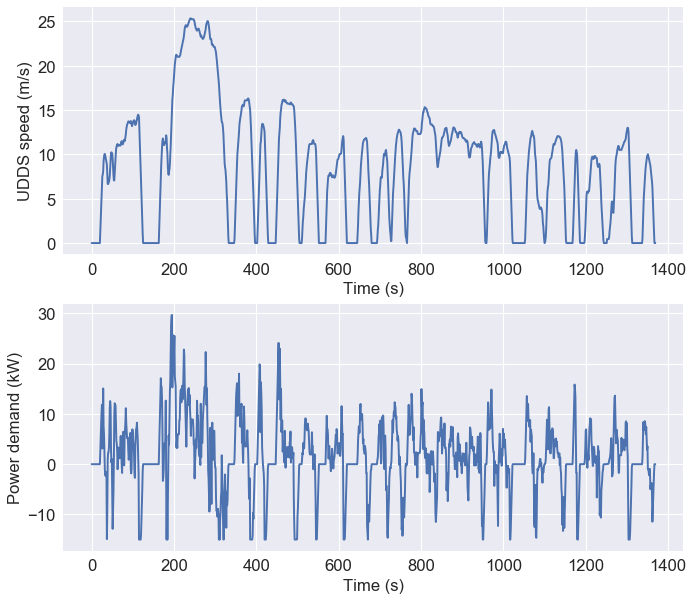
\includegraphics[width=\linewidth]{4a.png}     
	\caption{UDDS spped vs. time \& power demand vs. time}
\end{figure}
\newpage
\subsection{}
The plot is shown as follow:
\begin{figure}[H]
	\centering
	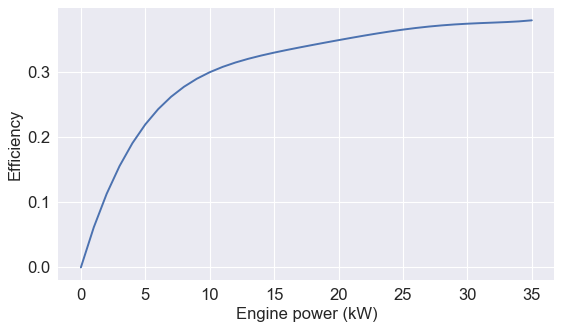
\includegraphics[width=\linewidth]{4b.png}  
	\caption{Engine efficiency curve}
\end{figure}
\section{}
\subsection{(b)\ \ \ (c)}
\begin{lstlisting}[language=Python]
## SOLVE DYNAMIC PROGRAM
start = timeit.timeit()

# Boundary Condition of Value Function (Principle of Optimality)
V[:,N] = 0

# Iterate backward in time
for k in range(N-1, -1, -1):

# Iterate over SOC
for idx in range(0,ns):

# Find dominant bounds for P_batt
lb = max(-P_batt_max, Qcap * V_oc / Delta_t * (SOC_grid[idx]-SOC_max), P_dem[k] - P_eng_max)
ub = min(P_batt_max, Qcap * V_oc / Delta_t * (SOC_grid[idx]-SOC_min), P_dem[k])

# Grid Battery Power between dominant bounds
P_batt_grid = np.linspace(lb,ub,200)

# Compute engine power (vectorized for all P_batt_grid)
P_eng = -P_batt_grid + P_dem[k]

# Cost-per-time-step, a.k.a. fuel consumed at each stage (vectorized for all P_batt_grid)
g_k = alph * Delta_t / eta_eng(P_eng) * P_eng

# compute next SOC using dynamics
SOC_nxt = SOC_grid[idx] - Delta_t / (Qcap * V_oc) * P_batt_grid

# Compute value function at nxt time step (need to interpolate)
V_nxt = interp(SOC_nxt, SOC_grid, V[:,k+1])

# Value Function (Principle of Optimality)
V[idx,k] = min(g_k + V_nxt)
ind = np.argmin(g_k + V_nxt)

# Save Optimal Control
u_star[idx,k] = P_batt_grid[ind]

# DP Timer
end = timeit.timeit()
print(str(end - start) + " seconds")
\end{lstlisting}
\newpage
\section{}
\subsection{}
\begin{lstlisting}[language=Python]
## Simulate Results

# Preallocate
SOC_sim = np.zeros((N,))
P_batt_sim = np.zeros((N,))
P_eng_sim = np.zeros((N,))
J_sim = np.zeros((N,))

# Initialize
SOC_0 = 0.75# put initial SOC here!
SOC_sim[0] = SOC_0

# Simulate PHEV Dynamics
for k in range(0,(N-1)):

# Use optimal battery power, for given SOC
P_batt_sim[k] = interp(SOC_sim[k], SOC_grid, u_star[:, k])

# Compute engine power
P_eng_sim[k] = P_dem[k] - P_batt_sim[k]

# Fuel Consumption
J_sim[k] = alph * Delta_t / eta_eng(P_eng_sim[k]) * P_eng_sim[k]

# Time-step SOC dynamics
SOC_sim[k+1] = -Delta_t / (Qcap * V_oc) * P_batt_sim[k] + SOC_sim[k]
\end{lstlisting}
\subsection{}
The minimum fuel consumption is just 0.
\newpage
\subsection{}
The plots are shown as follow:
\begin{figure}[H]
	\centering
	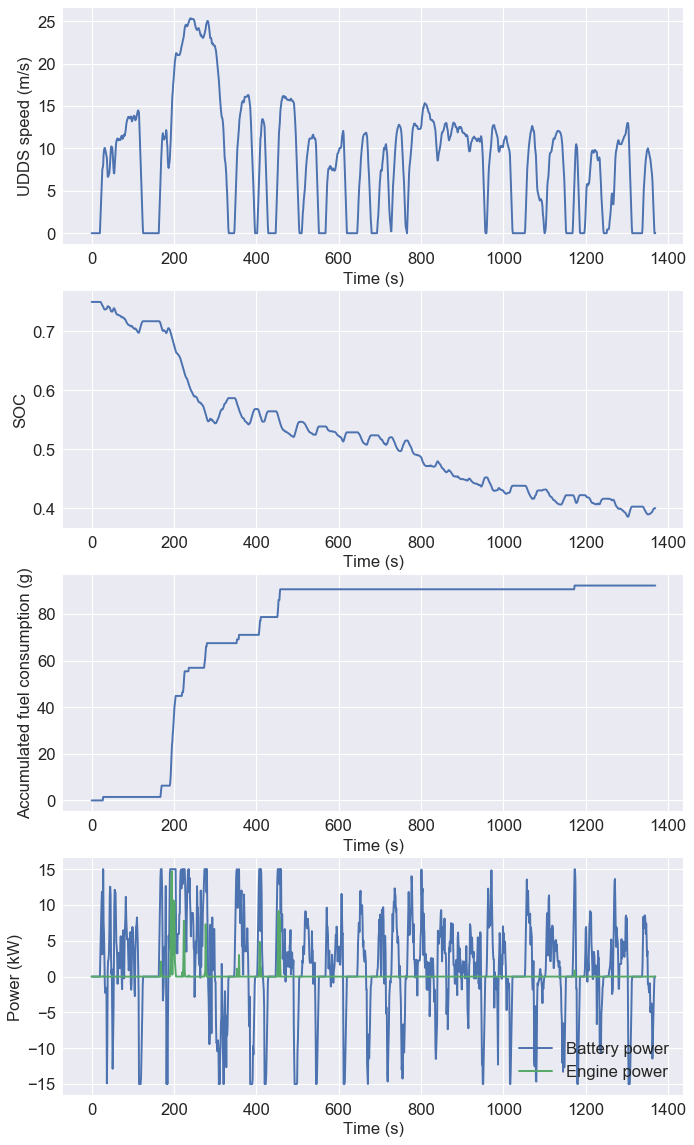
\includegraphics[width=12cm]{6c.png} 
	\caption{Data and result visualization}
\end{figure}
\subsection{}
Yes, all the inequality constraints are satisfied.
\section{}
We can change the initial SOC ``$SOC\_0$" in the code, and compute the simulated final SOC and total fuel consumption using the following script:
\begin{lstlisting}[language=Python]
SOC_sim[-1], np.cumsum(J_sim)[-1]/1000
\end{lstlisting}
The results are shown in Table 1.
\begin{table}[H]
	\caption{PHEV energy management results}
	\centering
	\begin{tabular}{cccc}
		\hline\hline
		\textbf{Initial SOC}&\textbf{Final SOC}&\textbf{Total Fuel Cons. (kg)}\\
		\hline
		0.9&0.55&0.09\\
		0.75&0.40&0.09\\
		0.6&0.27&0.13\\
		0.45&0.27&0.41\\
		0.3&0.27&0.65\\
		\hline\hline
	\end{tabular}
\end{table}
\section{}
From the result obtained in the previous problem, we notice that as the initial SOC decreases, the SOC trajectory decreases and finally remain unchanged (converged); while the total fuel consumption keeps increasing. I think the reason is that PHEV has the priority to use the electrical energy (battery) and use only a little fuel energy in the beginning. As battery SOC goes down to a certain level (0.27 shown in the result), fuel begins to be consumed as the main energy source to keep the battery in good conditions and avoid the low power issue.
\end{document}